\documentclass[11pt, a4paper]{article}

% Packages for formatting and functionality
\usepackage[utf8]{inputenc}
\usepackage[T1]{fontenc}
\usepackage{geometry}
\usepackage{xcolor}
\usepackage{listings}
\usepackage{hyperref}
\usepackage{graphicx}
\usepackage{booktabs}
\usepackage{enumitem}
\usepackage{titlesec}
\usepackage{palatino}
\usepackage{microtype} % Improves spacing when hyphenation is off
\usepackage{float}     % Forces table placement

% --- TIKZ PACKAGES FOR DIAGRAMS ---
\usepackage{tikz}
\usetikzlibrary{shapes, positioning, arrows.meta, shadows}

% Margins
\geometry{left=2.5cm, right=2.5cm, top=2.5cm, bottom=2.5cm}

% --- HYPHENATION SETTINGS ---
% Prevents words from breaking in the middle
\tolerance=1
\emergencystretch=\maxdimen
\hyphenpenalty=10000
\hbadness=10000

% Hyperlink setup
\hypersetup{
    colorlinks=true,
    linkcolor=black, % ToC links are black
    filecolor=magenta,      
    urlcolor=cyan,
    pdftitle={Intenus Whitepaper},
}

% Code Listing Configuration
\definecolor{codegreen}{rgb}{0,0.6,0}
\definecolor{codegray}{rgb}{0.5,0.5,0.5}
\definecolor{codepurple}{rgb}{0.58,0,0.82}
\definecolor{backcolour}{rgb}{0.95,0.95,0.92}

\lstdefinestyle{mystyle}{
    backgroundcolor=\color{backcolour},   
    commentstyle=\color{codegreen},
    keywordstyle=\color{magenta},
    numberstyle=\tiny\color{codegray},
    stringstyle=\color{codepurple},
    basicstyle=\ttfamily\footnotesize,
    breakatwhitespace=false,         
    breaklines=true,                 
    captionpos=b,                    
    keepspaces=true,                 
    numbers=left,                    
    numbersep=5pt,                  
    showspaces=false,                
    showstringspaces=false,
    showtabs=false,                  
    tabsize=2
}

\lstset{style=mystyle}

% --- RENAME LISTINGS ---
\renewcommand{\lstlistingname}{Snippet}

% --- LANGUAGE DEFINITIONS ---

% 1. TypeScript Definition
\lstdefinelanguage{TypeScript}{
  keywords={const, let, var, if, else, while, for, return, interface, class, extends, implements, public, private, protected, readonly, static, async, await, new, try, catch, throw, import, from, export, type, function, true, false, null, undefined, void, Promise, string, number, boolean, any},
  keywordstyle=\color{blue}\bfseries,
  ndkeywords={export, default, module},
  ndkeywordstyle=\color{darkgray}\bfseries,
  identifierstyle=\color{black},
  sensitive=true,
  comment=[l]{//},
  morecomment=[s]{/*}{*/},
  stringstyle=\color{codepurple}\ttfamily,
  morestring=[b]',
  morestring=[b]"
}

% 2. JSON Definition
\lstdefinelanguage{json}{
    basicstyle=\ttfamily\footnotesize,
    morestring=[b]",
    morecomment=[l]{//},
    literate=
     *{:}{{{\color{codegreen}{:}}}}{1}
      {,}{{{\color{codegreen}{,}}}}{1}
      {\{}{{{\color{blue}{\{}}}}{1}
      {\}}{{{\color{blue}{\}}}}}{1}
      {[}{{{\color{blue}{[}}}}{1}
      {]}{{{\color{blue}{]}}}}{1},
}

% 3. Move (Sui) Definition
\lstdefinelanguage{Move}{
  keywords={public, entry, fun, struct, module, use, has, store, drop, copy, u8, u64, vector, address, &mut, return, move, let, mut},
  keywordstyle=\color{blue}\bfseries,
  ndkeywords={self, Self},
  ndkeywordstyle=\color{darkgray}\bfseries,
  identifierstyle=\color{black},
  sensitive=true,
  comment=[l]{//},
  morecomment=[s]{/*}{*/},
  stringstyle=\color{red}\ttfamily,
  morestring=[b]"
}

% --- TITLE & METADATA ---
\title{\textbf{Intenus: Intent-Based DeFi Agent Infrastructure}}

% Author Block
\author{{Wynn Chill Lab} \\ \vspace{0.3em} \small \texttt{hello@intenus.xyz}}

% Date
\date{\small \today}

\begin{document}

\maketitle

\begin{abstract}
\noindent Intenus Protocol introduces a universal intent-based trading infrastructure powered by autonomous AI agents that transform natural language trading expressions into executable blockchain transactions. These intent-based AI agents operate within a decentralized network of verified solvers, coordinating through standardized representations defined by the Intenus General Standard (IGS). Each agent interprets, validates, and optimizes user intents, fostering competition to produce the most economically efficient execution strategy.

\vspace{0.5em}
\noindent To ensure trust-minimized coordination, solution verification and ranking are executed within Trusted Execution Environments (TEEs) utilizing the Nautilus Framework. By integrating Walrus for decentralized storage and Seal for programmable access control, Intenus establishes a unified, secure, and verifiable agent network that transcends traditional protocol boundaries and delivers optimal on-chain execution for users.

\vspace{1em}
\noindent \textbf{Keywords:} Intent-based AI agents, Intent-centric trading, Trusted execution environment, Decentralized solver network, AI-powered ranking, Programmable access control
\end{abstract}

\newpage
\tableofcontents
\newpage

\section{Introduction}

The decentralized finance ecosystem has evolved into a fragmented landscape where users must navigate multiple protocols, understand complex parameters, and execute transactions across disparate interfaces. Current intent-based protocols address specific use cases—primarily DEX aggregation—but lack the standardization and cross-protocol capability needed for comprehensive DeFi interactions.

Intenus Protocol addresses these limitations by introducing a Universal Solver Network (USN) that operates on standardized intent representations, enabling solvers to compete across all DeFi categories while maintaining verifiable execution quality through AI-powered ranking in trusted environments.

\subsection{Key Contributions}

The protocol introduces several foundational innovations to the DeFi landscape. The Intent General Standard (IGS) provides a comprehensive, extensible schema designed to standardize intent representation across spot trading, limit orders, lending, bridging, and complex DeFi operations.

Furthermore, Intenus implements Verifiable AI Ranking, utilizing advanced machine learning models for Intent Classification and reinforcement learning to determine primary actions and define scoring strategies for solution selection. This evaluation process is securely executed within Trusted Execution Environments (TEEs) using the Nautilus Framework, ensuring unbiased and optimal decision-making.

To ensure security and privacy, the system employs Programmable Access Control, integrating with Seal's encryption framework to enforce privacy-preserving mechanisms for handling sensitive intents and solver solutions. Finally, Decentralized Data Management is achieved by leveraging Walrus decentralized storage as a secure and efficient repository for archiving intents, solutions, and AI training data, ensuring cost-effective availability without compromising data integrity.

\section{Background and Motivation}

\subsection{Current State of Intent-Based Architectures}

Existing intent-based protocols suffer from several fundamental limitations that hinder broader adoption and efficiency. Protocol Fragmentation and Liquidity Silos remain a significant hurdle, as each protocol typically targets specific DeFi categories (e.g., CoW Protocol for DEX trading), requiring users to interact with multiple specialized platforms.

Additionally, the industry faces a Lack of Standardized Schema. The absence of a unified intent representation standard creates compatibility barriers, restricting solvers to specific protocols, stifling cross-protocol competition, and limiting the innovation of generalized solution strategies.

The ecosystem is also plagued by the Verifiability Dilemma, a trade-off between security and cost. On-chain verification of complex, non-deterministic solutions incurs prohibitive computational overhead and gas costs, while off-chain verification typically lacks trust guarantees, relying heavily on centralized intermediaries.

Finally, current systems rely on One-Dimensional Optimization. Solver selection mechanisms primarily optimize for simple deterministic metrics like lowest gas or maximum output. They lack sophisticated, multi-dimensional ranking mechanisms capable of evaluating qualitative factors such as historical solver reliability, complex user preferences, and risk-adjusted returns.

\subsection{Technical Opportunity}

The convergence of several Sui ecosystem technologies creates an opportunity for a fundamentally new approach. Sui's Programmable Transaction Blocks (PTBs) enable complex, atomic transaction composition that can execute multi-protocol strategies efficiently. The Nautilus TEE Infrastructure provides verifiable off-chain computation capabilities essential for AI-powered solution ranking. Walrus Decentralized Storage offers cost-effective storage for intent data, solutions, and training datasets while maintaining verifiability. Finally, Seal's Programmable Access Control enables sophisticated privacy controls for intent data and solver strategies.

\section{System Architecture}

\subsection{High-Level Overview}

Intenus Protocol operates as a four-layer architecture comprising the Application Layer (User-facing interfaces and Intent Agents), the Coordination Layer (Intent registry and solution orchestration), the Solver Layer (Decentralized network of competing solution providers), and the Infrastructure Layer (Nautilus TEE, Walrus storage, and Seal encryption).

% --- TIKZ DIAGRAM START ---
\begin{figure}[H]
\centering
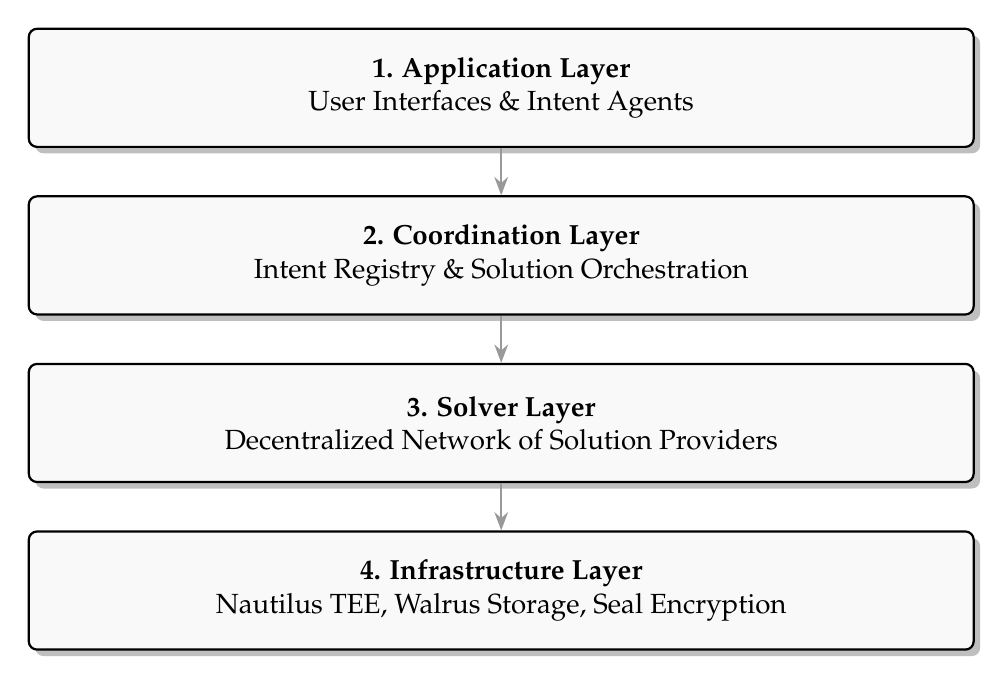
\begin{tikzpicture}[
    node distance=0.6cm,
    % Define the style for the boxes
    layer/.style={
        rectangle,
        draw=black,
        thick,
        fill=gray!5,
        align=center,
        minimum width=12cm, % Enforces same width for all rectangles
        minimum height=1.5cm,
        rounded corners=3pt,
        drop shadow
    },
    % Define style for arrows
    arrow/.style={
        ->,
        >=Stealth,
        thick,
        gray!80
    }
]

% 1. Application Layer
\node (app) [layer] {\textbf{1. Application Layer} \\ User Interfaces \& Intent Agents};

% 2. Coordination Layer
\node (coord) [layer, below=of app] {\textbf{2. Coordination Layer} \\ Intent Registry \& Solution Orchestration};

% 3. Solver Layer
\node (solver) [layer, below=of coord] {\textbf{3. Solver Layer} \\ Decentralized Network of Solution Providers};

% 4. Infrastructure Layer
\node (infra) [layer, below=of solver] {\textbf{4. Infrastructure Layer} \\ Nautilus TEE, Walrus Storage, Seal Encryption};

% Draw arrows to show dependency/flow
\draw [arrow] (app) -- (coord);
\draw [arrow] (coord) -- (solver);
\draw [arrow] (solver) -- (infra);

\end{tikzpicture}
\caption{Intenus Protocol Architectural Stack}
\label{fig:architecture}
\end{figure}
% --- TIKZ DIAGRAM END ---

\subsection{Core Workflow}

The system operates through a defined sequence of stages. First, Intent Submission occurs when users articulate trading goals via the Intent Agent, which transforms natural language or structured parameters into the standardized Intent General Standard (IGS) schema. This is immediately followed by Privacy Protection, where raw intent data is encrypted via Seal's programmable access control framework, enforcing granular visibility permissions to ensure only authorized solvers can decrypt specific fields.

During Solver Competition, registered solvers query available intents and compete to construct optimal execution paths, submitting their proposed solutions within a discrete auction window. Subsequently, AI-Powered Ranking is conducted within a Trusted Execution Environment (TEE) utilizing the Nautilus Framework. Inside this secure enclave, AI models execute Intent Classification and apply reinforcement learning-based scoring strategies to validate and rank solutions against multi-dimensional metrics such as profitability, risk, and reliability.

Finally, the process concludes with Verifiable Execution, where the protocol selects the optimal solution backed by a verifiable ranking proof. The transaction is executed on-chain, and relevant execution data is archived on Walrus for transparency and future model training.

\section{Standards and Specifications}

To ensure seamless interoperability between the Application Layer (User Intents), the Solver Network, and the AI Training Infrastructure, Intenus Protocol enforces strict data standardization. These standards are defined using JSON Schema Draft 07, ensuring that all system actors—from wallet clients to TEE-based ranking engines—adhere to a unified communication protocol.

\subsection{Intenus General Standard (IGS)}

The IGS Framework acts as the universal language for the protocol. It is composed of three hierarchical schema definitions designed to maximize modularity and extensibility.

\subsubsection{Core Primitive Definitions}

This schema defines the foundational data types used across the entire protocol. By standardizing primitives such as asset identifiers, numeric precision, and cryptographic signatures, we eliminate ambiguity in data parsing. The Purpose of this schema is to define reusable types (e.g., \texttt{SuiAddress}, \texttt{BigInt}, \texttt{Timestamp}, \texttt{Signature}). Validation enforces strict regex patterns for addresses and range checks for numeric values.

\begin{lstlisting}[language=json, caption=IGS Core Primitive Example]
{
  "igs_version": "1.0.0",
  "intent_type": "swap.exact_input",
  "operation": {
    "mode": "exact_input",
    "inputs": [{
      "asset_id": "0x2::sui::SUI",
      "amount": {"type": "exact", "value": "1000000000"}
    }],
    "outputs": [{
      "asset_id": "0x...::usdc::USDC",
      "amount": {"type": "range", "min": "950000", "max": "1000000"}
    }]
  },
  "constraints": {
    "max_slippage_bps": 50,
    "deadline_ms": 1699123456000
  }
}
\end{lstlisting}

\subsubsection{Intent Specification}

The Intent Schema governs how user requirements are expressed. It decouples the "what" (user goal) from the "how" (execution path). This schema supports polymorphism, allowing for various intent types (Swap, Limit, Bridge, Lending) within a single structure. Key features include Conditional Logic, which supports constraints like \texttt{min\_output}, \texttt{deadline}, and \texttt{max\_gas\_price}, and Access Control, which integrates Seal-specific fields for encrypted payloads.

\subsubsection{Solution Specification}

Solvers must submit solutions strictly adhering to this schema. This standardization is critical for the Nautilus TEE to deterministically simulate, validate, and rank competing solutions without bias. The components include an Execution Plan (the sequence of Move calls or PTBs), Simulation Results (expected output amounts and gas estimation), and a Solver Commitment (cryptographic signatures binding the solver to specific performance guarantees).

\subsection{Decentralized AI Data Standards}

To fuel the autonomous evolution of the Intenus AI Agents, all interaction data is archived on Walrus decentralized storage. This data serves as the ground truth for model retraining and performance auditing.

\subsubsection{Training Dataset Schema}

This schema defines the structure of historical data blobs stored on Walrus. It aggregates the Intent, the winning Solution, the execution outcome, and market context at the time of execution. Its Utility enables the AI to learn from past solver performance and user behaviors via Reinforcement Learning from Human Feedback (RLHF). Furthermore, Anonymization ensures that sensitive user data is stripped or hashed before being added to the public training set, compliant with privacy standards.

\section{Core Components}

\subsection{Universal Solver Network (USN)}

The USN enables heterogeneous solver strategies to compete on standardized intent representations.

\subsubsection{Solver Registration and Staking}

Solvers must register with minimum stake requirements and undergo reputation tracking:

% REPLACED CODE SNIPPET WITH TABLE
\begin{table}[H]
\centering
\renewcommand{\arraystretch}{1.2}
\begin{tabular}{@{} p{0.4\textwidth} p{0.6\textwidth} @{}}
\toprule
\textbf{Field} & \textbf{Description} \\ \midrule
\texttt{solver\_address} & Uniquely identifies the solver on-chain. \\
\texttt{stake\_amount} & The minimum stake required to participate in auctions. \\
\texttt{reputation\_score} & A dynamic score reflecting historical performance reliability. \\
\texttt{total\_batches\_participated} & Count of auction batches the solver has engaged in. \\
\texttt{accuracy\_score} & Metric measuring the precision of solver's past solutions. \\
\texttt{status} & Current operational status (e.g., Active, Suspended). \\ \bottomrule
\end{tabular}
\caption{Solver Profile Data Structure}
\label{tab:solver_profile}
\end{table}

\subsubsection{Solution Strategies}

Unlike constrained systems (e.g., CoW's P2P focus), USN supports diverse approaches. DEX Aggregation provides multi-hop routing optimization across AMMs, while P2P Matching performs intent coincidence of wants analysis for peer-to-peer settlement. The system also supports Hybrid Strategies combining on-chain execution with MEV capture, and AI-Driven Solutions utilizing machine learning-based strategy selection.

\subsection{AI-Powered Ranking Engine}

The ranking engine operates within Nautilus TEE infrastructure to ensure verifiable, unbiased solution evaluation.

\subsubsection{Intent Classification}

Machine learning models classify intents to determine optimal ranking strategies based on intent type, complexity, and market conditions.

\subsubsection{Multi-Factor Ranking}

Solutions are evaluated across multiple dimensions. Economic Efficiency is measured by surplus generation relative to benchmark expectations. Execution Quality assesses gas optimization and slippage minimization. Speed Metrics evaluate expected execution time and confirmation probability, while Solver Reputation considers historical performance and stake-weighted reliability.

\subsubsection{Verifiable Computation}

All ranking computations occur within attested TEE environments. This provides Attestation Proofs for cryptographic verification of computation integrity, ensures Deterministic Results for reproducible ranking given identical inputs, and guarantees Privacy Preservation so solution details remain confidential during evaluation.

\subsection{Privacy-Preserving Data Management}

\subsubsection{Seal Integration for Access Control}

Intenus leverages Seal's programmable access control for sophisticated privacy management:

% REPLACED CODE SNIPPET WITH TABLE
\begin{table}[H]
\centering
\renewcommand{\arraystretch}{1.2}
\begin{tabular}{@{} p{0.4\textwidth} p{0.6\textwidth} @{}}
\toprule
\textbf{Field} & \textbf{Description} \\ \midrule
\texttt{solver\_access\_window} & Defines the start and end timestamps for allowed access. \\
\texttt{requires\_solver\_registration} & Boolean flag enforcing verified solver status. \\
\texttt{min\_solver\_stake} & Minimum stake threshold required for decryption access. \\
\texttt{auto\_revoke\_time} & Timestamp for automatic revocation of access rights. \\ \bottomrule
\end{tabular}
\caption{Intent Policy Data Structure}
\label{tab:intent_policy}
\end{table}

Access policies ensure that only qualified solvers can decrypt intent data. They enforce time-bounded access to prevent stale solution submissions and implement automatic revocation to protect user privacy post-execution.

\subsubsection{Walrus Storage Integration}

Intent and solution data utilize Walrus's decentralized storage to achieve Cost Efficiency, as off-chain storage reduces transaction costs for large intent schemas. Data Integrity is maintained via cryptographic proofs ensuring data authenticity, while Availability Guarantees provided by distributed storage ensure access for time-sensitive intents.

\section{Security Model}

\subsection{Trust Assumptions}

Intenus operates under a defined trust model. On-Chain Security relies on Sui's consensus mechanism for transaction finality and state consistency. TEE Security trusts the Nautilus infrastructure for computation integrity, verified through remote attestation. Economic Security depends on solver stake amounts and slashing mechanisms to prevent malicious behavior, while Cryptographic Security utilizes Seal's encryption protocols for data confidentiality and access control.

\subsection{Attack Vectors and Mitigations}

\subsubsection{Solver Misbehavior}

The protocol actively mitigates solver misbehavior. MEV Extraction, where solutions extract value without benefiting users, is mitigated by AI ranking that detects unusual surplus patterns and penalizes violations via slashing. Stale Data Attacks, involving outdated market data, are prevented through timestamp validation in the TEE environment and strict recency requirements. Solution Copying is thwarted by requiring encrypted solution submissions and time-bounded access.

\subsubsection{Privacy Attacks}

Privacy attacks are addressed through robust encryption. Intent Frontrunning, using intent information for adversarial trading, is mitigated by Seal encryption with time-bounded solver access and automatic revocation. Solution Correlation, enabling the inference of strategies from public solution patterns, is prevented by privacy-preserving ranking in the TEE and differential privacy techniques.

\subsection{Slashing and Appeals}

The protocol implements sophisticated slashing mechanisms:

% REPLACED CODE SNIPPET WITH TABLE
\begin{table}[H]
\centering
\renewcommand{\arraystretch}{1.2}
\begin{tabular}{@{} p{0.35\textwidth} p{0.6\textwidth} @{}}
\toprule
\textbf{Field} & \textbf{Description} \\ \midrule
\texttt{batch\_id} & Unique identifier for the auction batch involved. \\
\texttt{solver\_address} & The on-chain address of the accused solver. \\
\texttt{severity} & Level of the infraction (e.g., Low, Medium, Critical). \\
\texttt{attestation} & Cryptographic proof of the violation from the TEE. \\
\texttt{tee\_measurement} & Verification of the TEE code state during execution. \\ \bottomrule
\end{tabular}
\caption{Slashing Evidence Data Structure}
\label{tab:slashing_evidence}
\end{table}

An appeals process allows solvers to challenge slashing decisions within 24-hour windows, with resolution provided by protocol governance.

\section{Economic Model}

\subsection{Incentive Structure}

\subsubsection{Solver Incentives}

Solvers are incentivized through Performance Rewards, where top-ranked solutions receive proportional fees from executed intents. They also engage in Reputation Building, as consistent performance increases reputation scores, leading to higher solution visibility. Furthermore, Stake Multipliers ensure that higher stake amounts provide competitive advantages in ranking algorithms.

\subsubsection{User Benefits}

Users gain significant advantages, including Optimized Execution via AI-powered ranking that ensures superior execution compared to direct protocol interaction. The system offers a Simplified UX, where natural language intent expression abstracts complex DeFi mechanics, and robust Privacy Protection, as encrypted intents prevent frontrunning and sandwich attacks.

\subsection{Fee Distribution}

Total fees collected from intent execution are distributed strategically, with Solver Rewards accounting for 90\% to selected solution providers, and 10\% allocated to the Protocol Treasury for infrastructure maintenance and development.

\subsection{Token Economics}

While Intenus operates on existing tokens (SUI for gas, individual assets for trading), the protocol introduces Reputation NFTs, which are soulbound tokens representing solver performance history, and Achievement Badges for recognition of milestone performance metrics. Future developments will include Governance Tokens for community governance of protocol parameters and upgrades.

\section{Related Work and Positioning}

\subsection{Comparison with Existing Protocols}

\begin{table}[H]
\centering
\begin{tabular}{@{}lllll@{}}
\toprule
\textbf{Protocol} & \textbf{Scope} & \textbf{Standardization} & \textbf{AI Integration} & \textbf{Privacy} \\ \midrule
CoW Protocol      & DEX Trading    & None                     & No                      & Limited          \\
1inch             & DEX Aggregation& None                     & No                      & No               \\
Anoma             & General Intents& Partial                  & No                      & Yes              \\ 
\textbf{Intenus}  & \textbf{Universal DeFi} & \textbf{IGS Standard} & \textbf{TEE-based AI} & \textbf{Seal Integration} \\ \bottomrule
\end{tabular}
\caption{Protocol Comparison}
\end{table}

\subsection{Academic Foundations}

The protocol builds upon research in Intent-Based Programming by extending declarative transaction models to DeFi contexts, and Mechanism Design through optimal auction theory for solution selection and fee distribution. It also leverages Trusted Computing via TEE applications in blockchain infrastructure and Privacy-Preserving ML for secure computation in ranking algorithms.

\section{Conclusion}

Intenus Protocol marks a paradigm shift in decentralized finance, transitioning the ecosystem from fragmented, manual interaction models to a unified, intent-centric infrastructure. By successfully harmonizing the Intenus General Standard (IGS) with autonomous AI agents, the protocol resolves the critical "Verifiability Dilemma," proving that complex, off-chain computation can be trusted, audited, and seamlessly executed on-chain.

The protocol's architecture serves as a testament to the power of the Sui ecosystem. By orchestrating the Nautilus Framework for TEE-based solution ranking, Walrus for immutable data availability, and Seal for programmable privacy, Intenus delivers a level of security and efficiency that existing EVM-based intent bridges cannot replicate. This technological convergence ensures that users no longer have to choose between the optimal execution of a centralized exchange and the self-custody of a decentralized network.

As the industry evolves towards an agent-centric economy, Intenus is positioned not merely as a trading tool, but as the foundational middleware for automated finance. The protocol's modular design and open SDKs invite developers to build atop a verified liquidity layer, fostering a positive feedback loop where solver competition drives down costs and enhances execution quality. Ultimately, Intenus establishes the gold standard for how AI agents and blockchain protocols coordinate to deliver value, setting the stage for the mass adoption of intelligent, automated DeFi.

\section*{Glossary}
\begin{table}[H]
\centering
\renewcommand{\arraystretch}{1.5} % Reduced spacing from 1.5 to 1.2
\begin{tabular}{@{} p{0.25\textwidth} p{0.65\textwidth} @{}}
\toprule

\textbf{Term} & \textbf{Definition} \\ \midrule
\textbf{CoW} (Coincidence of Wants) & A situation where two parties each have what the other wants, enabling direct peer-to-peer exchange without intermediate transactions. \\
\textbf{IGS} (Intenus General Standard) & The universal schema framework that standardizes intent representation across all DeFi operations within the Intenus Protocol. \\
\textbf{Intent} & A declarative expression of a user's desired outcome without specifying the execution path. \\
\raggedright \textbf{MEV} (Maximum Extractable Value) & The maximum value that can be extracted from block production in excess of standard block rewards and gas fees. \\
\raggedright \textbf{PTB} (Programmable Transaction Block) & Sui's atomic transaction composition feature that enables complex multi-operation transactions in a single execution. \\
\textbf{RLHF} (Reinforcement Learning from Human Feedback) & A machine learning technique that incorporates human feedback to improve model performance and alignment. \\
\textbf{Slashing} & The penalty mechanism that deducts staked tokens from misbehaving solvers as punishment for protocol violations. \\
\textbf{Solver} & An entity that competes to provide optimal execution strategies for user intents within the protocol. \\
\textbf{Soulbound Token} & A non-transferable NFT that represents identity, credentials, or reputation that cannot be sold or transferred. \\
\textbf{TEE} (Trusted Execution Environment) & A secure area of a processor that ensures code and data loaded inside are protected with respect to confidentiality and integrity. \\
\textbf{USN} (Universal Solver Network) & The decentralized network of competing solvers that operate on standardized intent representations within Intenus Protocol. \\ 
\bottomrule
\end{tabular}
\end{table}

\pagebreak

\begin{thebibliography}{99}

\bibitem{sui}
Sui Foundation. (n.d.). \textit{Sui Move Programming Language Reference}. Retrieved November 22, 2025, from \url{https://docs.sui.io/}

\bibitem{walrus}
Danezis, G., Giuliari, G., Kokoris Kogias, E., Legner, M., Smith, J.-P., Sonnino, A., \& Wüst, K. (2025). \textit{Walrus: An Efficient Decentralized Storage Network} (v2.0). Mysten Labs. \url{https://docs.wal.app/walrus.pdf docs.wal.app+2arXiv+2}

\bibitem{walrusblog}
Mysten Labs. (2024, June 18). \textit{Announcing Walrus: A Decentralized Storage and Data Availability Protocol}. Mysten Labs Blog. \url{https://www.mystenlabs.com/blog/announcing-walrus-a-decentralized-storage-and-data-availability-protocol}

\bibitem{walruslaunch}
Mysten Labs. (2025, March 27). \textit{Walrus Launches on Mainnet, Unlocking Programmable Storage for All}. Mysten Labs Blog. \url{https://www.walrus.xyz/blog/public-mainnet-launch}

\bibitem{seal}
Mysten Labs. (2025, September 3). \textit{Seal Mainnet Launch: Bringing Data Privacy and Access Control to Web3}. Mysten Labs Blog. \url{https://www.mystenlabs.com/blog/seal-mainnet-launch-privacy-access-control}

\bibitem{sealweb}
Mysten Labs. (n.d.). \textit{Seal: Data Encryption and On‑chain Access Control}. Retrieved November 22, 2025, from \url{https://seal.mystenlabs.com/}

\bibitem{nautilus}
Sui Foundation. (2025, May 8). \textit{Introducing Nautilus: Bringing Verifiable Off-chain Privacy to Sui}. Sui Blog. \url{https://blog.sui.io/nautilus-offchain-security-privacy-web3/}

\bibitem{nautilusdocs}
Sui Foundation. (n.d.). \textit{Nautilus: Trusted Execution Environment}. Retrieved November 22, 2025, from \url{https://docs.sui.io/concepts/cryptography/nautilus}

\bibitem{anoma}
Anoma Research. (2023, September 28). \textit{An Introduction to Intents and Intent-Centric Architectures}. \url{https://anoma.net/blog/an-introduction-to-intents-and-intent-centric-architectures}

\bibitem{anomaresource}
Heuer, M., \& Reusche, D. (2024, August 26). \textit{Intent-centric Applications for the Anoma Resource Machine}. Zenodo. \url{https://doi.org/10.5281/zenodo.13340448}

\bibitem{anomawhitepaper}
Anoma project. (n.d.). \textit{Anoma: A Unified Architecture for Full-Stack Decentralised Applications}. Retrieved November 22, 2025, from the Anoma whitepaper: \url{https://media.githubusercontent.com/media/anoma/whitepaper/main/whitepaper.pdf}

\end{thebibliography}

\end{document}